\documentclass{article}
\usepackage{amsmath}
\usepackage{amssymb}
\usepackage{graphicx}
\usepackage{hyperref}
\usepackage[version=4]{mhchem}


\begin{document}
In \(\triangle A B C, A B=7 . A C=11 . A D\) is the median on side \(B C\). How many integer values are there of \(A D\) ?

Solution: 6.\\
\centering
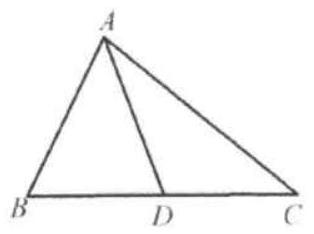
\includegraphics[width=\textwidth]{images/024(3).jpg}


Extend \(A D\) to \(E\) such that \(A D=D E\).\\
Connect \(B E\).

Since \(D E=A D, \angle B D E=\angle C D A . B D=D C\).\\
Thus \(\triangle B D E \cong \triangle C D A, B E=A C=11\).

By the triangle inequality theorem,\\
\centering
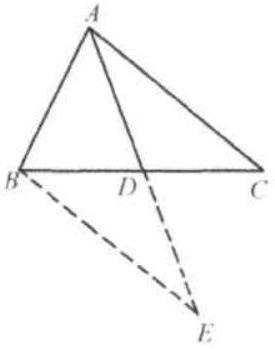
\includegraphics[width=\textwidth]{images/025(1).jpg}\\
\(11-7<A E<11+7 \Rightarrow 4<2 A D<18 \Rightarrow \quad 2<A D<9\).\\
There are six possible values: \(3,4,5,6,7\), and 8 .


\end{document}
